\section{Disjoint windows of entropy gain}\label{sec:windows}

Proposition~\ref{prop:pair-bands} supplies a linear amount of fair-pair
weight in a finite interval of logarithmic depths for every sufficiently long block
segment.  We now turn this weight into entropy gain.  The difficulty is
that the depth interval may extend arbitrarily far.  We choose several
segments whose depth intervals are separated, and show that their gains
occupy disjoint windows of block indices.  At each physical scale the
total gain is bounded, whereas every chosen interval contributes the same
positive amount after averaging over scales.

Throughout this section, retain the environment and constants from
Section~\ref{sec:types}.  Thus $\sigma_j=-\log|R_j|$ is the contraction
depth after $j$ blocks, $D$ bounds each block's depth, and
$\mathcal F_j=\sigma(\omega_0,\ldots,\omega_{j-1})$ records the first
$j$ types.  In particular, $\sigma_j\le Dj$.  The logarithmic-depth bands are
$[a_n,B_n]$, where $a_n=\lceil An\rceil-1$, and their expected total
weight on $E_n=\{\sigma_n\le A'n\}$ is at least $cn$.

Let $\theta$ denote the left shift of the type sequence.  Define the
suffix laws, including their contraction from the initial scale, by
\[
 \tau_j=\mathsf D_{R_j}\mu_{\theta^j\omega},\qquad j\ge0.
\]
The independent conditional block draws give the pathwise identity
\begin{equation}\label{eq:suffix-convolution}
 \tau_j=(\mathsf D_{R_j}\nu_{\theta^j\omega,n})*\tau_{j+n},
 \qquad n\ge1.
\end{equation}
All these laws have compact support.  The signs of $R_j$ are retained in
the laws; only scale changes use $|R_j|$.

By Lemma~\ref{lem:nonsaturation}, choose $\delta>0$ such that
\[
 \Delta_v(\mu):=1-G_{v,2v}(\mu)\ge\delta\qquad(v>0).
\]
Fix an integer $M>4$ with $5/M<\delta/2$.  For an integer target depth
$L\ge1$, write $r=2^{-L}$ and define
\begin{equation}\label{eq:window-entropy}
 g_j=G_{r/M,Mr}(\tau_j).
\end{equation}
Here and below $g_j$ depends on $L$ and $\omega$.  The ratio of the two
window scales is the integer $M^2$.  Lemma~\ref{lem:entropy-calculus}
and \eqref{eq:suffix-convolution} therefore imply, for every environment,
\begin{equation}\label{eq:window-monotonicity}
 0\le g_j\le2\log M,\qquad g_j\ge g_{j+1}.
\end{equation}

\subsection{A gain after averaging the unobserved future}

An individual conditional tail need not satisfy the nonsaturation bound
for $\mu$.  To use that bound, we condition only on the types through
the end of the finite block segment producing a fair pair.  The
unobserved future types then average its tail law back to a scaled copy
of $\mu$.

\begin{lemma}[Conditional pair gain]\label{lem:conditional-gain}
For all integers $j\ge0$, $n\ge1$, and $L\ge1$, with $g_j$ as in
\eqref{eq:window-entropy},
\begin{equation}\label{eq:conditional-gain}
 \E\bigl[g_j-g_{j+n}\mid\mathcal F_{j+n}\bigr]
 \ge \frac{\delta}{2}
 c_{L-\lceil\sigma_j\rceil}(\nu_{\theta^j\omega,n}).
\end{equation}
\end{lemma}

\begin{proof}
Condition on $\mathcal F_{j+n}$ and put
$\ell=L-\lceil\sigma_j\rceil$.  The finite law
$\nu_{\theta^j\omega,n}$, the signed products $R_j,R_{j+n}$, and
$\ell$ are now fixed.  Choose a fair-pair decomposition attaining
$c_\ell(\nu_{\theta^j\omega,n})$.  Such a choice is measurable in
$\mathcal F_{j+n}$: for fixed $j,n,L$ there are only finitely many
initial type sequences, so one may fix a maximizer for each of them.

A selected pair of distance $u\in[2^{-\ell},2^{1-\ell})$ has distance
$v=|R_j|u$ after scaling.  Since $r=2^{-L}$,
\[
 \frac vr\in
 \bigl[2^{\lceil\sigma_j\rceil-\sigma_j},
       2^{1+\lceil\sigma_j\rceil-\sigma_j}\bigr)
 \subset[1,4).
\]
Thus $r/M<v<Mr$ and
\[
 \frac{r/M}{v}+\frac{v}{Mr}\le\frac5M.
\]
Even if $R_j$ is negative, the scaled pair, after ordering its endpoints,
is a translate of the fair law on $\{0,v\}$.  Translation invariance
and Lemma~\ref{lem:two-point} show that this pair increases the window
entropy of $\tau_{j+n}$ by at least
\[
 \Delta_v(\tau_{j+n})-\frac5M.
\]

The types beginning at index $j+n$ are independent of
$\mathcal F_{j+n}$.  Since averaging $\mu_\omega$ over the environment
gives $\mu$, their conditional mean is the identity of measures
\[
 \E[\tau_{j+n}\mid\mathcal F_{j+n}]
   =\mathsf D_{R_{j+n}}\mu.
\]
The functional $\Delta_v=1-G_{v,2v}$ is convex by
Lemma~\ref{lem:entropy-calculus}.  Each chosen distance $v$ is fixed
under the present conditioning.  Hence Jensen's inequality and signed
scaling give
\begin{align*}
 \E[\Delta_v(\tau_{j+n})\mid\mathcal F_{j+n}]
 &\ge\Delta_v(\mathsf D_{R_{j+n}}\mu)\\
 &=\Delta_{v/|R_{j+n}|}(\mu)\ge\delta.
\end{align*}

Apply concavity of $G_{r/M,Mr}$ to the selected pairs and the residual
positive measure in the prefix law.  If the residual mass is nonzero,
normalize it to a probability law; convolution with that law contributes
a nonnegative gain by Lemma~\ref{lem:entropy-calculus}, since the scale
ratio is $M^2$.  The same statement is vacuous when the residual mass is
zero.  Summing the conditional lower bounds for all the selected pairs
therefore gives
\[
 \E[g_j-g_{j+n}\mid\mathcal F_{j+n}]
 \ge\left(\delta-\frac5M\right)
       c_\ell(\nu_{\theta^j\omega,n})
 \ge\frac\delta2c_\ell(\nu_{\theta^j\omega,n}),
\]
as required.
\end{proof}

\subsection{Choosing disjoint block windows}

Fix any positive integer $q$.  Choose sufficiently large integers
$n_1<\cdots<n_q$ successively so that
Proposition~\ref{prop:pair-bands} applies, $a_{n_i}\ge1$, and
\begin{equation}\label{eq:separated-bands}
 a_{n_i}-A'n_i-1>B_{n_h}\qquad(h<i).
\end{equation}
This is possible because the previously chosen $B_{n_h}$ are finite and
\[
 a_n-A'n-1=\lceil An\rceil-A'n-2
 \ge(A-A')n-2\longrightarrow\infty.
\]
In particular, the choice uses no upper bound on how fast $B_n$ grows.
Call $[a_{n_i},B_{n_i}]$ band $i$.  Larger $i$ means finer physical
scales, since \eqref{eq:separated-bands} gives $a_{n_i}>B_{n_h}$ for $h<i$.

Choose an even integer $T$ with
\begin{equation}\label{eq:target-range}
 \frac T2>\max_{1\le i\le q}B_{n_i}.
\end{equation}
For band $i$, use the candidate starts
\begin{equation}\label{eq:candidate-starts}
 J_i=\left\{kn_i:k\in\mathbb Z,\ 0\le k\le
                  \left\lfloor\frac{T}{2Dn_i}\right\rfloor\right\}.
\end{equation}
For each target $L\in\{1,\ldots,T\}$, retain the window
$[j,j+n_i)$, $j\in J_i$, exactly on the event
\begin{equation}\label{eq:retention}
 \mathcal A_{i,j,L}=
 \left\{\sigma_{j+n_i}-\sigma_j\le A'n_i,\quad
 a_{n_i}\le L-\lceil\sigma_j\rceil\le B_{n_i}\right\}.
\end{equation}
This event belongs to $\mathcal F_{j+n_i}$, the same sigma-algebra as
the conditioning in Lemma~\ref{lem:conditional-gain}.

The reason for the separation condition is simple.  As a block start
$j$ moves forward, the adjusted target depth
$L-\lceil\sigma_j\rceil$ is nonincreasing.  A retained window in a finer
band cannot decrease this depth far enough to reach any coarser band.
The next lemma makes this order precise for every environment.

\Needspace{5\baselineskip}
\begin{lemma}[Disjoint retained windows]\label{lem:disjoint-windows}
For each fixed environment and target $L\in\{1,\ldots,T\}$, all the
retained windows in \eqref{eq:retention} are pairwise disjoint.
Consequently,
\begin{equation}\label{eq:telescoping-windows}
 \sum_{i=1}^q\sum_{j\in J_i}
 \mathbf1_{\mathcal A_{i,j,L}}(g_j-g_{j+n_i})
 \le2\log M.
\end{equation}
\end{lemma}

\begin{proof}
Set $x_j=L-\lceil\sigma_j\rceil$; this is nonincreasing in $j$.
If the band-$i$ window $[j,j+n_i)$ is retained, then
\[
 \lceil\sigma_{j+n_i}\rceil-\lceil\sigma_j\rceil
 \le\sigma_{j+n_i}-\sigma_j+1\le A'n_i+1,
\]
so
\begin{equation}\label{eq:window-end-depth}
 x_{j+n_i}\ge a_{n_i}-A'n_i-1.
\end{equation}
If $[k,k+n_h)$ is a retained window in a coarser band $h<i$, then
$x_k\le B_{n_h}$.  By \eqref{eq:separated-bands} and
\eqref{eq:window-end-depth},
\[
 x_{j+n_i}>B_{n_h}\ge x_k.
\]
Monotonicity of $x_j$ forces $k>j+n_i$.  Thus the window from the finer band
ends before the window from the coarser band starts.  Within a single band,
distinct starts are distinct multiples of its length $n_i$, so its
half-open windows also do not overlap.

List the retained windows in increasing order as
$[u_1,v_1),\ldots,[u_N,v_N)$, with $v_t\le u_{t+1}$.  By
\eqref{eq:window-monotonicity},
\[
 \sum_{t=1}^N(g_{u_t}-g_{v_t})
 \le g_{u_1}-g_{v_N}\le2\log M.
\]
The empty sum is zero.  This proves \eqref{eq:telescoping-windows}.
\end{proof}

Figure~\ref{fig:disjoint-windows} shows the order of retained windows
from two different bands in this proof.

\begin{figure}[t]
\centering
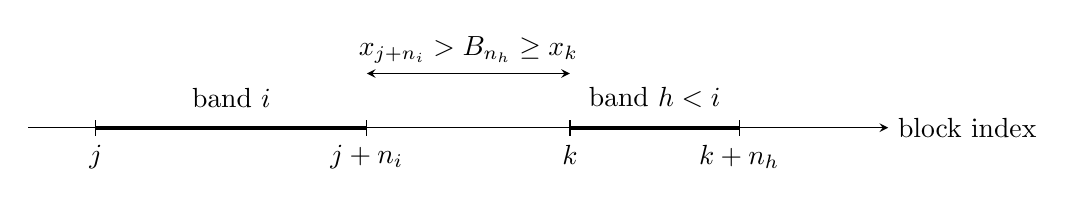
\begin{tikzpicture}[x=0.86cm,y=0.86cm,>=stealth]
 \draw[->] (0,0)--(12.7,0) node[right] {block index};
 \draw[line width=1.5pt] (1,0)--(5,0);
 \draw[line width=1.5pt] (8,0)--(10.5,0);
 \foreach \x in {1,5,8,10.5}{\draw (\x,-0.12)--(\x,0.12);}
 \node[below] at (1,-0.12) {$j$};
 \node[below] at (5,-0.12) {$j+n_i$};
 \node[below] at (8,-0.12) {$k$};
 \node[below] at (10.5,-0.12) {$k+n_h$};
 \node[above] at (3,0.15) {band $i$};
 \node[above] at (9.25,0.15) {band $h<i$};
 \draw[<->] (5,0.8)--(8,0.8);
 \node[above] at (6.5,0.8) {$x_{j+n_i}>B_{n_h}\ge x_k$};
\end{tikzpicture}
\caption{At a fixed target depth, a retained window from a finer band
ends before any retained window from a coarser band begins.  Here
$x_j=L-\lceil\sigma_j\rceil$ is nonincreasing in the block index.  The
schematic is not to scale.}
\label{fig:disjoint-windows}
\end{figure}

\subsection{Summing over target depths}

The disjointness lemma bounds the total gain at one physical scale.
Summing over targets recovers every pair scale in each band.  Indeed,
for a candidate $j\in J_i$,
\[
 0\le\sigma_j\le Dj\le T/2.
\]
Because $T$ is even, this also gives
$0\le\lceil\sigma_j\rceil\le T/2$.  Each integer
$\ell\in[a_{n_i},B_{n_i}]$ therefore occurs exactly once as
$L-\lceil\sigma_j\rceil$ for $1\le L\le T$: take
$L=\ell+\lceil\sigma_j\rceil$.  Its lower bound is $1$, and its
upper bound is at most $B_{n_i}+T/2<T$.

Each band has at least $T/(2Dn_i)$ candidate starts, and each contributes
expected pair mass at least $cn_i$ after summing the targets.  The block
length cancels, so every band supplies a fixed multiple of $T$.
Take expectations in \eqref{eq:telescoping-windows}.  Since the retention
indicator is $\mathcal F_{j+n_i}$-measurable, the tower property and
Lemma~\ref{lem:conditional-gain} apply to each summand.  Sum the result
over $L=1,\ldots,T$ and use the preceding exact correspondence to obtain
\begin{align}
 2T\log M
 &\ge\frac\delta2\sum_{i=1}^q\sum_{j\in J_i}
 \E\left[
 \mathbf1_{E_{n_i}}(\theta^j\omega)
 \sum_{\ell=a_{n_i}}^{B_{n_i}}
 c_\ell(\nu_{\theta^j\omega,n_i})\right]
 \notag\\
 &\ge\frac{\delta c}{2}\sum_{i=1}^q |J_i|n_i
 \ge\frac{\delta c qT}{4D}.
 \label{eq:final-window-count}
\end{align}
The second inequality uses Proposition~\ref{prop:pair-bands} and the
identical distribution of the type environment under $\theta^j$;
independence between different candidate windows is not needed.  The
last inequality follows from the exact count
\[
 |J_i|=\left\lfloor\frac{T}{2Dn_i}\right\rfloor+1
 \ge\frac{T}{2Dn_i}.
\]
After canceling $T$, \eqref{eq:final-window-count} bounds the arbitrary
integer $q$ by $8D\log M/(\delta c)$.  All the constants in this bound
were fixed before $q$ was chosen, so this is impossible.

\begin{proof}[Completion of the proof of Theorem~\ref{thm:main}]
The standard upper bound gives
$\dim_H\mu\le\min\{1,h/\chi\}$.  If the inequality were strict,
then $d=\dim_H\mu$ would satisfy $d<1$ and $d\chi<h$.
Section~\ref{sec:types} would supply the pair bands used above, and
\eqref{eq:final-window-count} would give a contradiction.  Therefore
$\dim_H\mu=\min\{1,h/\chi\}$ for the prescribed positive vector
$p$.  Since $p$ was arbitrary, the conclusion holds for every such
vector, including the cases $h=\chi$ and $h>\chi$.
\end{proof}
